\section{High Performance Implementation}

We undertake two classes of high performance implementations for the CX method. We start with a highly optimized, close-to-the-metal C implementation that focuses on obtaining peak efficiency from conventional multi-core CPU chipsets. The purpose of this exercise is to establish a baseline for the CX method. Secondly, we implement the CX method in Spark, an emerging standard for parallel data analytics frameworks. Implementing the method in Spark provides us with a scalable strategy to run on multiple nodes, and tackle a large scale dataset. 


\label{sec:implementation}

     \begin{figure*}[htp]
         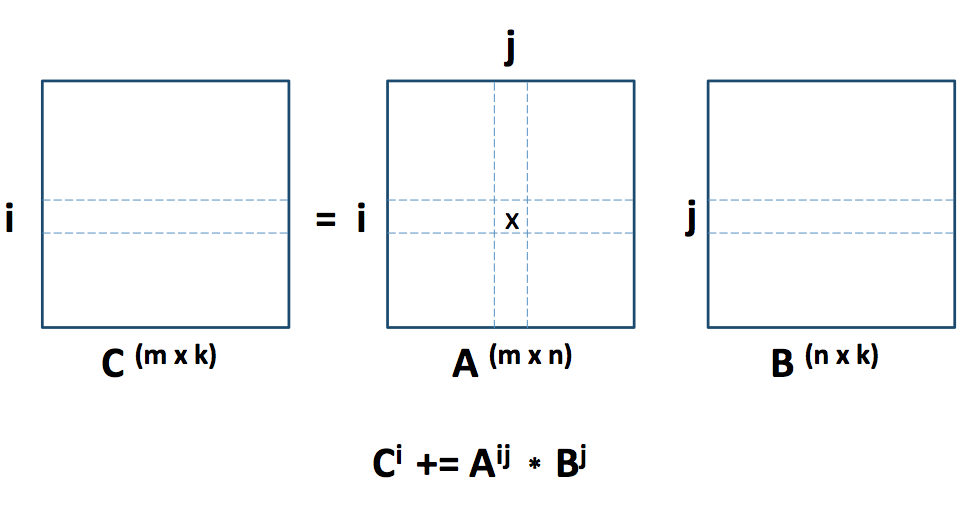
\includegraphics[scale=0.254]{images/jatin_a}
         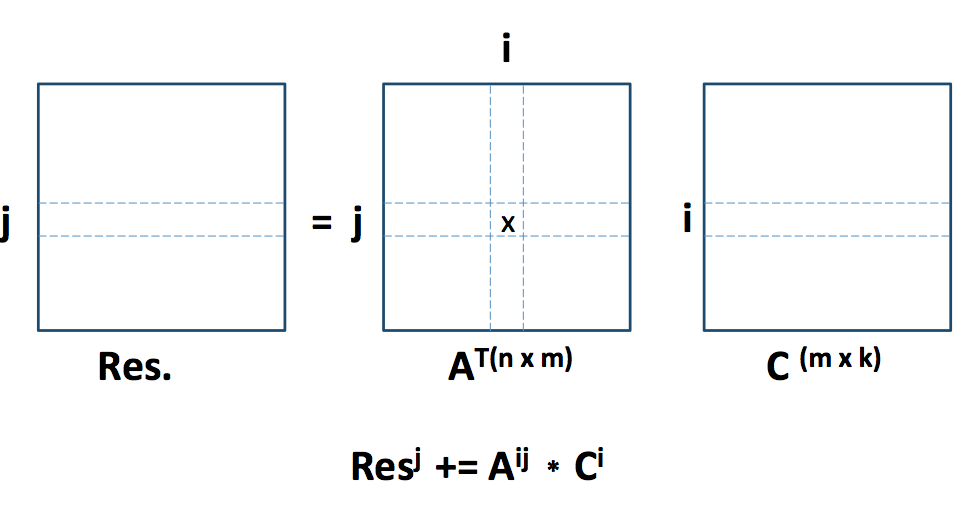
\includegraphics[scale=0.254]{images/jatin_b}
         \caption{ Data access pattern for computing ${C}_{\it{i}}$ (left) and {\it{Res}}$_{\it{j}}$ (right) respectively.}
         \label{fig:access_pattern}
           \end{figure*}


\subsection {Single Node Implementation/Optimizations}
\label{sxn:single_node_opt}

    We now focus on optimizing the CX implementation on a single
    compute-node, aimed at exploiting the available SIMD units on each
    core, and the multiple cores across different sockets to speed up the performance. 
    We began by profiling our initial %%unoptimized 
    scalar serial CX
    code and optimizing the steps in the order of execution times.
    The max. time is spent in computing sparse-sparse-dense matrix
    multiplication ($A^TAB$, Step 3, 91.2\%), followed by  sparse-dense matrix
    multiplication ($AQ$, Step 7, 8.6\%) and finally, QR
    decomposition (Step 4, 0.2\%)
    for a representative dataset that fits in main memory. These
    {\it{three}} kernels account for more than 99.9\% of
    the execution time.
    Recall that $A$ is a sparse matrix with dimensions ({\it{m}} X
    {\it{n}}) and sparsity {\it{s}}, and B is a dense ({\it{n}} X {\it{k}}) matrix.
    We first discuss the case of $A^TAB$.

\vspace*{0.1in} 
{\bf{{ {Optimizing $A^TAB$:}}}}
    Optimizing sparse matrix-matrix  multiplication continues to be an
    active area of research~\cite{ballard13,patwary15}, with focus on
    reducing communication, and the state of the art implementations
    are bound by the memory bandwidth and heavily
    underutilize the compute resources. 
    %%
    %%As far as computing $A^TAB$ is concerned, 
    For our application, we exploit the following {\it{three}} observations:
    (1) One of the sparse matrices is the transpose of the other,   
    (2) One of the matrices is a dense matrix,   and    %%The sparse-sparse matrix multiplication is followed by a sparse-dense matrix multiplication. 
    (3) ({\it{n}} $\gg$  {\it{k}} and  {\it{sm}} $\gg$ {\it{k}}).

    Exploiting associativity of multiplication, we perform $C$ = $AB$, 
    followed by $Res =$ $A^TC$. This reduces the run-time complexity from
    O({\it{n*(nsm)}}) to O({\it{k*(nsm)}}). Furthermore, we do not
    explicitly compute (or store) the transpose of A.  Consider the
    ${\it{i}}^{th}$ row of A (A$_{\it{i}}$). 
    By definition, 
    C$_{\it{i}}$ %(1 X {\it{k}}) 
    = A$_{\it{i}}$$\cdot$$B$.
     The (${\it{j}},{\it{l}}$)$^{th}$ element of Res,
    Res$_{{\it{j}},{\it{l}}}$ =
    $\Sigma_{\it{p}}$($A^T_{{\it{j}},{\it{p}}}$ x $C$$_{{\it{p}},{\it{l}}}$) = 
    $\Sigma_{\it{p}}$($A_{{\it{p}},{\it{j}}}$ x
    $C$$_{{\it{p}},{\it{l}}}$).
%% 
%% 
%% 
%% 
    For {\it{p}} = {\it{i}}, this reduces to incrementing
    Res$_{{\it{j}},{\it{l}}}$ by $A_{{\it{i}},{\it{j}}}$ x
    $C$$_{{\it{i}},{\it{l}}}$. 
%% 
%% 
%% 
    Thus, for each row {\it{i}}, 
    %having computed C$_{\it{i}}$, we can scale each entry by  $A_{{\it{i}},{\it{j}}}$ 
    having computed C$_{\it{i}}$, we
    increment Res$_{{\it{j}},{\it{l}}}$ 
    by $A_{{\it{i}},{\it{j}}}$ x $C$$_{{\it{i}},{\it{l}}}$
    for {\it{j}}$\in$[1..{\it{n}}] and {\it{l}}$\in$[1..{\it{k}}].
     We now describe how we parallelize this algorithm to exploit
     data- and thread-level parallelism and other relevant
     optimizations.

     %%%%%%%%%%%%%%%%%%%%%%%%%%%%%%%%%%%%%%%%%%%%%%%%%%%%%%%%%%%%%%%%%%%%%%%%%%%%%%%%%%%%%%%%%%%%%%%%%%%%%%%%%%%%%%%%%%%%%




     %%%%%%%%%%%%%%%%%%%%%%%%%%%%%%%%%%%%%%%%%%%%%%%%%%%%%%%%%%%%%%%%%%%%%%%%%%%%%%%%%%%%%%%%%%%%%%%%%%%%%%%%%%%%%%%%%%%%%
     %%%%%%%%%%%%%%%%%%%%%%%%%%%%%%%%%%%%%%%%%%%%%%%%%%%%%%%%%%%%%%%%%%%%%%%%%%%%%%%%%%%%%%%%%%%%%%%%%%%%%%%%%%%%%%%%%%%%%
     \vspace*{0.1in}
     {\it{1. Exploiting SIMD}}: Refer to Fig.~\ref{fig:access_pattern}. 
     Consider element $A_{{\it{i}},{\it{j}}}$. To compute
     $C_{\it{i}}$, we need to scale each element of
     $B_{{\it{j}}}$ by  $A_{{\it{i}},{\it{j}}}$ and add it to
     $C_{\it{i}}$ ({\it{j}}$\in$[1..{\it{n}}]) ($C_{\it{i}}$ +=
     $A_{{\it{i}},{\it{j}}}$ x $B_{{\it{j}}}$). Note that there are
     {\it{k}} elements in $B_{{\it{j}}}$, which are also stored
     consecutively (matrix stored in a row-major fashion).
%%
     On modern computing platforms, SIMD width (number of simultaneous
     operations that can be performed) is
     growing~\cite{intel1,intel2}. SSE can perform 4
     single-precision floating point operations in a single op., while
     AVX (our SPARK platform) performs 8 ops. Let $\mathcal{S}$ denote the SIMD width
     (defined as number of double-precision floating point ops. per op
     -- which is half of single-precision ops).
    %% 
     The pseudo-code~\footnote{Exact syntax varies with the ISA and
     compiler version.} for computing $C_{\it{i}}$ ($\forall$ $A_{{\it{i}},{\it{j}}}$ $\neq$ 0)
     \vspace*{0.05in}

     \hspace*{-0.0in}xmm\_a = {\it{vec\_load\_and\_splat}}($A_{{\it{i}},{\it{j}}}$); \\
     for\hspace*{0.02in}({\it{z}} = 0; {\it{z}} $<$ {\it{k}}; {\it{z}} += $\mathcal{S}$)\\
     \{\\
         \hspace*{0.2in}xmm\_c = {\it{vec\_load}}  ($C_{{\it{j}}}$ + z); \\
         \hspace*{0.2in}xmm\_b = {\it{vec\_load}}  ($B_{{\it{j}}}$ + z); \\
         \hspace*{0.2in}xmm\_ab = {\it{vec\_mul}}  (xmm\_a, xmm\_b); \\
         \hspace*{0.2in}xmm\_c = {\it{vec\_add}}  (xmm\_ab, xmm\_c); \\
         \hspace*{0.2in}{\it{vec\_store}} (xmm\_C,  $C_{{\it{j}}}$ + z); \\
     \}\\

     As evident from the self explanatory code, for each
     $A_{{\it{i}},{\it{j}}}$ $\neq$ 0 ({\it{nnz}} in total in matrix $A$), 
     we execute ($\lceil$$\frac{k}{\mathcal{S}}$$\rceil$) 
     {\it{add}} (and same number of {\it{mul}}) operations -- for a
     total of
     $\lceil$$\frac{2*{\it{nnz}}*{\it{k}}}{\mathcal{S}}$$\rceil$ operations,
     a potential speedup of $\mathcal{S}$,  
     in terms of floating point operations executed.

     We now describe the vectorization for computing $Res =$ $A^TC$.
     Note that $C$ is a dense matrix. As explained above, this
     requires incrementing Res$_{{\it{j}}}$ 
     by $A_{{\it{i}},{\it{j}}}$ x $C$$_{{\it{i}}}$ 
     (both Res$_{{\it{j}}}$ and $C$$_{{\it{i}}}$ have {\it{k}} elements each.)
    We execute a similar code to the previous step, to perform 
    $\lceil$$\frac{2*{\it{nnz}}*{\it{k}}}{\mathcal{S}}$$\rceil$
    operations,
    a potential speedup of $\mathcal{S}$,
    in terms of floating point operations executed.

    On some architectures, vector loads and stores are faster if
    memory addresses are 256-bit (or 512-bit aligned). 
    Since all our memory loads/stores start with each row of any
    matrix, we assign {\it{k}}  to be a multiple of 8, and align the
    starting addresses of all matrices to take advantage of such
    scenarios.
    

     %%%%%%%%%%%%%%%%%%%%%%%%%%%%%%%%%%%%%%%%%%%%%%%%%%%%%%%%%%%%%%%%%%%%%%%%%%%%%%%%%%%%%%%%%%%%%%%%%%%%%%%%%%%%%%%%%%%%%
     %%%%%%%%%%%%%%%%%%%%%%%%%%%%%%%%%%%%%%%%%%%%%%%%%%%%%%%%%%%%%%%%%%%%%%%%%%%%%%%%%%%%%%%%%%%%%%%%%%%%%%%%%%%%%%%%%%%%%
     %%%%%%%%%%%%%%%%%%%%%%%%%%%%%%%%%%%%%%%%%%%%%%%%%%%%%%%%%%%%%%%%%%%%%%%%%%%%%%%%%%%%%%%%%%%%%%%%%%%%%%%%%%%%%%%%%%%%%

     \vspace*{0.1in}
     {\it{2. Exploiting multiple cores}}: As explained above, we
     decompose the matrix multiplication into two steps, %each for each row of $C$$_{{\it{i}}}$, 
     we {\it{first}} compute
     $C$$_{{\it{i}}}$ ({\it{k}} elements), followed by updating 
     Res$_{{\it{j}}}$ for each row {\it{j}}. The number of executed 
     flops (and memory loads/stores) is proportional to number of
     non-zeros in the specific row of $A$. Thus a straightforward way
     to divide work equally between the various computing cores
     ($\mathcal{C}$ in total) is to divide the rows between the cores
     such that each of them perform work on the same number of {\it{nnz's}}. However,
     this might result in some of the rows being split between cores.
     For reasonable sized matrices, it suffices to assign a complete
     row to a core, without any slowdown.

     Thus each core (or thread) computes the starting and ending row
     index, and for each assigned row {\it{i}}, computes
     $C$$_{{\it{i}}}$. Now, the next step is to update Res.
%%
     Two different possibilites exist. One option is for each thread
     to maintain a local copy of $Res$, and once all the threads are
     done executing, reduce the results to form the final answer.
     However, even for moderately sized datasets, (e.g. $k$ = 32,
     {\it{n}} = 32K, and 8-bytes/element amounts to around
     4MB/thread), 
     {\it{far exceeds}} the last level cache per core.
     Hence, with this approach, for each assigned row,  would load and store the
     complete $Res$ matrix. A more efficient approach is to maintain a
     single copy of $Res$ shared by all the threads executing on a
     single-node, locks are used as described next. 

     We initialize {\it{n}} locks, one for each row of the output
     matrix ($Res$).
     %%, and each thread grabs a lock, performs update to a row of the matrix, and releases the lock.
     Once an executing thread computes $C$$_{{\it{i}}}$ (as the first
     step of the matrix multiplication 
     for an assigned row {\it{i}}), 
     for each  $A_{{\it{i}},{\it{j}}}$ $\neq$ 0, it grabs the
     ${\it{j}}^{th}$ lock, updates the row, and releases the lock. 
     %
     For realistic datasets, for sparsity({\it{s}})
     ($\sim$
     0.001 -- 0.005), there is a very low probability of two threads
     blocking on a lock$\sim$1\% even with ${\mathcal{C}}$ =
     128. We show in the results section that the contention indeed is
     very low, and most of the parallelization overhead is due to the
     instruction overhead for grabbing and releasing the locks.

     %%%\Comment{Jatin}{What is the instruction overhead for grabbing alock?}

     %%%%%%%%%%%%%%%%%%%%%%%%%%%%%%%%%%%%%%%%%%%%%%%%%%%%%%%%%%%%%%%%%%%%%%%%%%%%%%%%%%%%%%%%%%%%%%%%%%%%%%%%%%%%%%%%%%%%%
     %%%%%%%%%%%%%%%%%%%%%%%%%%%%%%%%%%%%%%%%%%%%%%%%%%%%%%%%%%%%%%%%%%%%%%%%%%%%%%%%%%%%%%%%%%%%%%%%%%%%%%%%%%%%%%%%%%%%%
     %%%%%%%%%%%%%%%%%%%%%%%%%%%%%%%%%%%%%%%%%%%%%%%%%%%%%%%%%%%%%%%%%%%%%%%%%%%%%%%%%%%%%%%%%%%%%%%%%%%%%%%%%%%%%%%%%%%%%
     \vspace*{0.1in}
     {\it{3. Cache Blocking}}: For smaller values of {\it{n}}, our
     thread-level parallelization scheme scales near-linearly with
     increasing number of cores. However, for {\it{n}} $>$ 64K, we
     started noticing a drop in scaling. This is due to the working
     set growing larger than the size of the last-level cache, and
     thereby the computation becoming bound by the available memory
     bandwidth. In contrast, if most of the memory fetches can come
     from the caches, we can efficiently  utilize the floating
     point compute units on the node. We now
     describe the computation of the working set, and our algorithm
     for performing cache-friendly updates.

     During the execution of the algoritm, the matrix $B$ is
     accessed, which is shared between all the cores. Matrix $A$ is a
     streaming read from the memory, and does not contribute to
     the working set. Let's say each thread maintains  its local copy
     of the $Res$ matrix, thereby the total working set being
     8{\it{kn}}*($\mathcal{C}$ + 1) bytes. For our system
     architecture, with $\mathcal{C}$ = 24, and matrix parameters of
     {\it{k}} = 32 and {\it{n}} = 128K, the total working set becomes
     around 1 GB, which is too large to fit in the
     caches~\footnote{In this discussion, caches refers to the last
     level cache}. Instead,
     maintaining a shared copy of the $Res$ matrix reduces it to
     8{\it{kn}} bytes, around 128 MB for this example. Note that the
     total size is indepent of the number of cores, and thus future
     proofs our implementation w.r.t. increasing number of cores on a
     single node. However, it is still dependent on {\it{n}}, the
     number of columns in the input matrix $A$, and thus we devise the
     following scheme to reduce it further to a given cache size of
     the computing platform.

     Instead of performing the computation for {\it{n}} columns, we
     divide it into chunks of {\it{n}}$'$ columns, such that
     2*8*{\it{k}}*{\it{n}}$'$ $\sim$ $\mathcal{C}$. Hence, with
     $\mathcal{C}$ = 15 MB,  {\it{n}}$'$$\sim$ 64K elements (we set
     {\it{n}} to be a multiple of {\it{n}}$'$ for ease of
     implementation). We thus perform the computation in
     $\lceil\frac{\it{n}}{\it{n}'}\rceil$ rounds, 
     updating the corresponding rows
     ([{\it{r}}$\lceil\frac{\it{n}}{\it{n}'}\rceil$..({\it{r}} +
     1)$\lceil\frac{\it{n}}{\it{n}'}\rceil$]
     in round {\it{r}}).
     Recall from the previous subsection that the number of flops
     executed per {\it{nnz}} element in $A$ is
     $\lceil\frac{4{\it{k}}}{\mathcal{S}}\rceil$.
     Since the non zeros elements of $A$ are stored consecutively, 
     this may require loading each element
     $\lceil\frac{\it{n}}{\it{n}'}\rceil$ times. Hence, the flops/byte
     of the computation is around
     $\lceil\frac{4{\it{k}}}{\mathcal{S}}\rceil$/$\lceil\frac{\it{n}}{\it{n}'}\rceil$.
     Using our representative numbers, this is around 16 flops/byte,
     which is greater than the peak flops/byte of the platform (around
     10 flops/byte), and
     hence our application is not bound by memory bandwidth. With
     large values of {\it{n}}, we might end up being bandwidth bound
     -- in which case we need to modify the way $A$ is stored, by
     storing it in chunks of columns that would be accessed in each
     round. This format of representing $A$  helps 
     exploit the complete computational power of the processor, 
     %%keep the computation bound by the compute flops, 
     and only incurs a
     one-time cost of rearranging  the elements of $A$.
     {\it{n}}$'$ = 64K seems to be a resonable chunk size for current
     architectures.

     %%%%%%%%%\Comment{Jatin}{How to store A might be an interesting way -- Say like n = 64K}.
     
     %%%%%%%%%%%%%%%%%%%%%%%%%%%%%%%%%%%%%%%%%%%%%%%%%%%%%%%%%%%%%%%%%%%%%%%%%%%%%%%%%%%%%%%%%%%%%%%%%%%%%%%%%%%%%%%%%%%%%
     %%%%%%%%%%%%%%%%%%%%%%%%%%%%%%%%%%%%%%%%%%%%%%%%%%%%%%%%%%%%%%%%%%%%%%%%%%%%%%%%%%%%%%%%%%%%%%%%%%%%%%%%%%%%%%%%%%%%%
     %%%%%%%%%%%%%%%%%%%%%%%%%%%%%%%%%%%%%%%%%%%%%%%%%%%%%%%%%%%%%%%%%%%%%%%%%%%%%%%%%%%%%%%%%%%%%%%%%%%%%%%%%%%%%%%%%%%%%

     \vspace*{0.1in}
     {\it{4. Multi-socket Optimization}}: 
     Multi-socket architectures are increasing being used for
     high-performance computing, wherein each socket has its own
     compute and memory resources. It is indeed possible for cores in
     any socket to access data present in the memory of the other
     sockets. However, all cross-socket traffic goes through a
     cross-socket link, which has lower bandwidth than access to local
     DRAM and caches. Hence, we need to optimize the amount of data
     transferred between sockets to ensure optimal performance.

     For our current application, in order to reduce the inter-socket
     communication, we divide the allocaton of $Res$ equally between
     the sockets. For e.g., for a CPU with 2 sockets, we divide the
     number of rows ({\it{n}}) by 2, and allocate the memory for each
     relevant part of the matrix on its individual socket. This
     ensures that (at an average), each socket has similar number of
     remote memory accesses. For our experiments, the
     prescribed style of memory allocation provided a boost of
     $\sim$5 -- 10\% to our performance, but we expect the optimizaton
     to be more beneficial with increasing number of
     sockets~\cite{fdsfds}.
     
     
     %%Current CPU dies have more than one socket~\cite{fds}.

     %%Given {it{k}}, and cache size $\mathcal{C}$, we desire 2 copies of the matrix to reside in cache -- hence, 
%%     As explained above, we decompose the matrix multiplication into two steps, %each for each row of $C$$_{{\it{i}}}$, 

%%%%%%%%%%%%%%     $A_{{\it{i}},{\it{j}}}$ $\neq$ 0 ({\it{nnz}} in total in matrix $A$), 

%%     https://software.intel.com/sites/landingpage/IntrinsicsGuide/


%%%%%%%     \vspace*{0.3in}


    
    %%As explained in Sec.~\ref{sec:5.1?}, 



    %ballard -- Communication Optimal Parallel Multiplication of Sparse Random Matrices
    %http://www.eecs.berkeley.edu/~odedsc/papers/spaa13-sparse.pdf

\vspace*{0.1in} 
{\bf{{ {Optimizing $AB$:}}}}

    This step refers to Step 7 in the algorithm description in
    Sec.~\ref{sec:cx_spark}. The data- and thread-level paralleization optimizations described 
    in the previous subsection (optimizing $A^TAB$) apply here, since
    there we explicitly  compute $C$ = $AB$. As far as cache blocking is
    concerned, since $C$ does not have to be memory resident, we now have
    to ensure that $B$ is completely cache resident (i.e. $8nk\le
    \mathcal{C}$). With increasing {\it{n}}, we again peform the
    computation in multiple rounds, with each round operating on 
    $n'=\frac{\mathcal{C}}{8k}$ rows of $B$.
%%
%%
%%%, and compute {\it{n}}$'$ (the number of columns of  accordingly. 
    Finally, as far as multi-socket optimizations are concerned, we
    divide the allocation of $C$, the output matrix in this case,
    between the various sockets, to reduce the amount of cross-socket
    memory traffic.





\iffalse
\begin{itemize}
\item Cache-Friendly 
\item SIMD
\item Thread- or core-level
\item Multi-socket 
\end{itemize}
\fi

\subsection{Spark}

To support operating on datasets larger than can be stored and processed on a single node,
we implement the algorithms using the Apache Spark cluster computing framework.

Spark provides a high-level programming model and execution engine for
fault-tolerant parallel and distributed computing, based on a core 
abstraction called a \textit{resilient distributed dataset (RDD)}.
Each RDD may be thought of as a distributed collection of objects that is
partitioned and stored across the Spark cluster.
RDDs are immutable lazily materialized collections supporting functional
programming operations such as \texttt{map}, \texttt{filter}, and \texttt{reduce},
each of which returns a new RDD.
RDDs may be loaded from a distributed file system, computed from other RDDs,
or created by parallelizing a collection created within the user's application.
RDDs of key-value pairs may also be treated as associative arrays, supporting
operations such as \texttt{reduceByKey}, \texttt{join}, and \texttt{cogroup}.
For example, to compute word frequencies of a text dataset in HDFS:
\begin{verbatim}
val dataset: RDD[String] =
      spark.textFile("hdfs://...")

val counts: RDD[(String, Int)] =
      dataset.
      flatMap(line => line.split(" ")).
      map(word => (word, 1)).
      reduceByKey(_ + _)

val countsMap: Map[String, Int] =
      counts.collectAsMap
\end{verbatim}

Spark employs a lazy evaluation strategy for efficiency.
All Spark operations that have no immediate side-effects other than returning an RDD are deferred
if possible.
Instead, deferrable operations simply create an entry in the program's DAG, recording the input
dependencies and capturing any closures and values needed.
This approach allows Spark to defer computations as much as possible, and when the evaluation
is unavoidable the entire Spark job can be examined by Spark's scheduler.
This allows the Spark execution engine to batch together related operations, optimize data locality,
and perform better scheduling.
A major benefit of Spark over MapReduce is the use of in-memory caching and storage so that data structures
may be reused rather than being recomputed.

\subsection{Multi-node CX and PCA implementation on Spark}
\label{sec:cx_spark}
The main consideration when implementing CX and PCA in a parallel setting are
efficient implementations of operations involving the data matrix $A$.
All access of $A$ by the CX and PCA algorithms occurs through the
\textsc{RandomizedSVD} routine shared in common.
\textsc{RandomizedSVD} in turn accesses $A$ only through the \textsc{MultiplyGramian} and
\textsc{Multiply} routines, with repeated invocations of \textsc{MultiplyGramian}
accounting for the majority of the algorithm's execution time.

The matrix $A$ is stored as an RDD containing one \texttt{IndexedRow} per row of the input matrix,
where each \texttt{IndexedRow} consists of the row's index and corresponding data vector.
This is a natural storage format for many datasets stored on a distributed or shared file
system, where each row of the matrix is formed from one record of the
input dataset, thereby preserving locality by not requiring data shuffling
during construction of $A$.

We then express \textsc{MultiplyGramian} in a form amenable to efficient distributed implementation
by exploiting the fact that the matrix product $A^TAB$ can be written as a sum of outer products,
as shown in Algorithm \ref{alg:gram}. This allows for full parallelism across the rows of the matrix with
each row's contribution computed independently, followed by a summation step to accumulate the result.
This approach may be implemented in Spark as a \texttt{map} to form the outer products followed by a \texttt{reduce}
to accumulate the results:
\begin{verbatim}
def multiplyGramian(A: RowMatrix, B: LocalMatrix) =
  A.rows.map(row => row * row.t * B).reduce(_ + _)
\end{verbatim}
However, this approach forms $2m$ unnecessary temporary matrices of same dimension as the output matrix $n\times k$,
with one per row as the result of the \texttt{map} expression, and the \texttt{reduce} is not done in-place so it
too allocates a new matrix per row.
This results in high GC pressure and makes poor use of the CPU cache, so
we instead remedy this by accumulating the results in-place by replacing the \texttt{map}
and \texttt{reduce} with a single \texttt{treeAggregate}.
The \texttt{treeAggregate} operation is equivalent to a map-reduce that executes in-place to accumulate the contribution of a
single worker node, followed by a
tree-structured reduction that efficiently aggregates the results from each worker.
The reduction is performed in multiple stages using a tree topology to avoid creating a single
bottleneck at the driver node to accumulate the results from each worker node.
Each worker emits a relatively large result with dimension $n\times k$, so the
communication latency savings of having multiple reducer tasks is significant.
\begin{verbatim}
def multiplyGramian(A: RowMatrix, B: LocalMatrix) = {
  A.rows.treeAggregate(LocalMatrix.zeros(n, k))(
    seqOp = (X, row) => X += row * row.t * B,
    combOp = (X, Y) => X += Y
  )
}
\end{verbatim}




